\section{METODOLOGI}

% Ubah konten-konten berikut sesuai dengan isi dari metodologi

\subsection{Data dan Peralatan}

\subsubsection{Data}
Dataset yang akan digunakan dalam proses pembuatan tugas akhir ini yaitu dataset buatan peneliti. Adapun rencana pembuatan dataset yaitu dataset berdasarkan beberapa tulisan tangan dari rekan peneliti yang ditulis disebuah papan tulis dan kemudian diambil gambarnya dalam beberapa pengaturan sudut, resolusi, serta pencahayaan yang berbeda.

\subsubsection{Peralatan}
\begin{itemize}
   \item [a.] Laptop \\
   Laptop merupakan perangkat keras (Hardware) yang berfungsi untuk mengolah data. Laptop yang digunakan pada penelitian tugas akhir memiliki spesifikasi Intel Core i5-8300H 2.3 GHz (8 CPUs), HDD Storage 1 TB, SSD Storage 256 GB, RAM 16 GB DDR4 2666 MHz, Graphic Card NVIDIA GeForce GTX 1050 Ti 4GB GDDR5.
   \item [b.] Google Colaboratory \\
   Google Colaboratory merupakan sebuah \textit{cloud-based executable code} yang dapat menunjang programmer dalam menjalankan serangkaian kode yang dimilikinya. Keunggulan dari Google Colaboratory yaitu proses eksekusi kode dapat dilakukan secara cloud sehingga dapat meringankan beban kerja pada laptop.
\end{itemize}
   

\subsection{Metodologi Penelitian}
Metodologi yang digunakan dalam pengerjaan Tugas Akhir ini adalah sebagai berikut.
    % Contoh input gambar dengan format *.jpg
    \begin{figure} [H] \centering
      % Nama dari file gambar yang diinputkan
      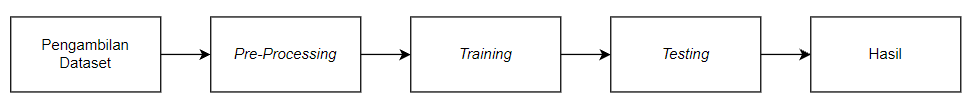
\includegraphics[scale=0.6]{gambar/Metodologi.png}
      % Keterangan gambar yang diinputkan
      \caption{Diagram blok metodologi}
      % Label referensi dari gambar yang diinputkan
      \label{fig:Metodologi}
    \end{figure}

\begin{enumerate}
   \item \textbf{Pengambilan Dataset} \\
   Pada tahapan ini, dilakukan proses pengambilan data berdasarkan kebutuhan pembuatan tugas akhir. Data yang akan dikumpulkan pada tahapan ini yaitu berupa sejumlah foto dari masing-masing huruf balok. Adapun dataset ini rencananya akan memiliki 26 kelas yang masing-masing mewakili huruf alfabet balok. Pada tahapan ini pula, dilakukan proses pemberian label pada dataset.
   \item \textbf{Pre-Processing} \\
   Pada tahapan ini, dilakukan \textit{pre-processing} dari dataset yang sebelumnya telah didapat. Pada tahapan ini pula, dataset dibagi menjadi 3 bagian yaitu \textit{data training, data validation dan data testing.}
   \item \textbf{Training} \\
   Pada tahapan ini, dilakukan proses \textit{training} dan \textit{tuning} menggunakan YOLO. Pada proses ini pula ditentukan \textit{epoch, Batch Size,} dan jenis model YOLO yang akan digunakan.
   \item \textbf{Testing} \\
   Pada tahapan ini, dilakukan proses testing yaitu untuk pengujian model yang telah dibangun sebelumnya untuk menentukan apakah model yang telah dibuat dirasa sudah cukup atau perlu dilakukan perubahan konfigurasi kembali dari awal. Pada tahapan ini pula, model dianalisa serta dievaluasi menggunakan \textit{Confusion Matrix.}
   \item \textbf{Hasil} \\
   Pada tahapan ini, jika model telah sesuai dengan threshold dan model telah berfungsi dengan baik, maka proses selanjutnya yaitu pelaporan dalam pembukuan tugas akhir.
\end{enumerate}